\documentclass[acmtog]{acmart}

\usepackage{lipsum}
\usepackage{url}
% \usepackage[colorlinks=true, citecolor=blue]{hyperref}

\AtBeginDocument{%
  \providecommand\BibTeX{{%
    Bib\TeX}}}

\setcopyright{cc}
\copyrightyear{2025}

\hypersetup{
    colorlinks=true,
    citecolor=blue,
    linkcolor=black,
    urlcolor=black
}

\begin{document}

\title{Computational Co-Design by Morphological Control Optimization}
\subtitle{Research, Teaching and Valorization Proposal of within Computational Dynamics Group}

\author{Brandon Caasenbrood}
% \authornote{}
\email{{b.j.caasenbrood@gmail.com}}
\orcid{1234-5678-9012}
\authornotemark[1]
% \affiliation{%
%   \institution{Eindhoven University of Technology}
%   \city{Eindhoven}
%   \state{North Brabant}
%   \country{the Netherlands}
% }

\renewcommand{\shortauthors}{Caasenbrood et al.}

\begin{abstract}
\textbf{Research abstract:} Traditional mechatronic system design has
predominantly adhered to a sequential, ad-hoc methodology in which the
physical structure and control are developed independently. In this
conventional paradigm, mechanical design decisions are typically
finalized prior to the integration of control architecture, frequently
overlooking the co-dependent interactions between structural dynamics
and control performance. Such segregated philosophy may leed in
suboptimal system behavior, as the interdependencies between mechanical
and control domains are not systematically addressed during its design
process. On the other hand, \emph{computational concurrent design}---or
\emph{co-design}---enables the parallel optimization of both mechanical
structure and control algorithms. This integrated methodology enhances
overall system performance and adaptability, particularly in
high-precision applications where the interaction between structure and
control is of paramount importance. By leveraging on the methods of
co-design, the proposed research framework addresses the limitations of
traditional design approaches: suboptimal system performance,
disturbance attenuation, suboptimal sensor and actuator placement,
lacking adaptability under operational conditions, and low lifetime.

This research proposes a dynamic topology optimization framework for
high-precision mechatronics and robotics. By extending density-based
methods to include temporal evolution, the framework enables concurrent
optimization of structure and control. Multi-indexed density variables
represent material distribution, actuator placement, and time-dependent
control inputs, facilitating efficient co-design. The approach aims to
advance the design and performance of next-generation mechatronic
systems.

\end{abstract}

\keywords{Computational Co-Design, Morphological Control, Optimization, Computational Dynamics}

% \begin{teaserfigure}
%   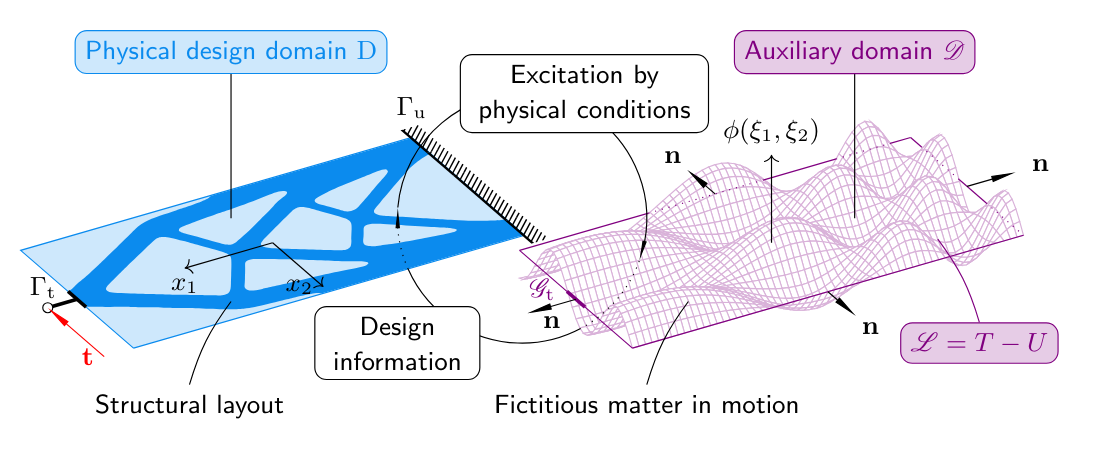
\includegraphics[width=0.75\textwidth]{image.png}
%   \caption{}
%   % \Description{Enjoying the baseball game from the third-base
%   % seats. Ichiro Suzuki preparing to bat.}
%   \label{fig:teaser}
% \end{teaserfigure}

% \received{20 February 2007}
% \received[revised]{12 March 2009}
% \received[accepted]{5 June 2009}

% \vspace{-40mm}
\maketitle

\section*{\textbf{Research on computational co-design}}

\textbf{What is co-design?} Co-design refers to the integrated process
of simultaneously optimizing both the physical structure that endows its
function (morphology) and the control strategies of a system. Early
examples of co-design include the pioneering works by Sims
\cite{sims1994evolving,sims1991artificial} in the early 90s, which
demonstrated the generative design of locomoting virtual creatures.
Here, both the morphologies of the virtual organisms and their
neuro-muscular control systems were evolved together using genetic
algorithms. Over the past three decades of research, catalyzed by the
persistent advancements in computational processing, the co-design has
branched into a interdisciplinary research domain
\cite{mirzendehdel2023codesign}. Notably, recent years have witnessed
significant increase in co-design methodologies for (soft) robotic
systems
\cite{sato2023topology,sato2024computational,allison2013plantlimited,bravopalacios2020one}.

\textbf{Open challenges}. Despite its recent academic resurgence,
several critical shortcomings continue to limit its potential
applicability.

First, co-design techniques are often burdened by high computational
demands during optimization, which can hinder effective exploration of
the design space. For example, in structural optimization with control
feedback \cite{yuhn20234d,sato2024computational,strgar2025accelerated},
the system is frequently modeled as a time-dependent Partial
Differential Equations (PDE). Traditionally, each optimization iteration
requires explicit discretization of the spatial domain, followed by
numerically solving the resulting discrete system over its relevant
spatial and then temporal horizon, respectively. This sequential process
is computationally expensive, especially as dimensionality of the design
space increase. Recent advances have sought to address these challenges
by representing the geometry of the spatial domain implicitly, such as
through level-set methods or neural implicit representations (see neural
PDE-refiner \cite{lippe2023pderefiner, li2020fourier}). These approaches
enable parametric design, where geometric modifications are encoded as
continuous parameters, facilitating smooth and flexible exploration of
the design space. Moreover, implicit representations enable direct PDE
surrogate solutions without rediscretization, reducing computational
overhead and supporting efficient optimization of complex,
high-dimensional geometries in multidisciplinary co-design.

Second, there remains a significant gap on how to tailor \emph{``good
metrics''} related to \emph{``good designs.''} The issue here is
twofold. On one hand, it is desirable to define metrics that are both
computationally efficient and tractable, such that it facilitates fast
evaluation and numerical adaptivity in the optimization process. On the
other hand, these metrics must also capture vital aspects of design,
e.g., manufacturability and design constraints, production cost, product
lifespan and maintainability, robustness, and compliance with regulatory
standards. The balance between computational tractability and practical
relevance often necessitates a hierarchical or multi-fidelity approach:
initial optimization may rely on simplified, computationally inexpensive
metrics to broadly explore the design space and avoid premature
convergence to local minima, followed by progressive refinement using
higher-fidelity, more computationally intensive evaluations that
gradually improving design confidence.

Third, a persistent challenge in co-design is the disparity between
simulation-based design (sim) and real-world deployment (real), commonly
referred to as the \emph{``Sim2Real} gap. This gap arises due to
modeling inaccuracies, unmodeled dynamics, and inherent
oversimplifications of simulation environments in favor of computation,
which can result in suboptimal or even infeasible designs when
transferred to physical systems. Recent advances in data-driven modeling
offer promising avenues to mitigate these discrepancies. By leveraging
empirical data collected from real-world experiments, data-driven
approaches can refine simulation models, improve parameter estimation,
and adapt control strategies to better reflect actual system behavior.

Finally, the inherently multidisciplinary nature of co-design
necessitates the involvement of diverse stakeholders throughout the
entire design process. However, current state-of-the-art co-design
methodologies frequently fall short in systematically integrating input
from a broad range of perspectives or adequately addressing the full
spectrum of its end-user requirements.

\section*{\textbf{Proposed research framework}}

\textbf{Problem statement.} To underscore the significance of co-design
as a methodological framework, consider the illustrative design
scenarios depicted in Fig. 1 and Fig. 2. The first example addresses a
disturbance-rejection problem, which is particularly relevant in
high-precision industries such as semiconductor manufacturing. The
second example focuses on the design of a docking interface, with
applications in space engineering and advanced robotics. These cases
exemplify the diverse challenges that co-design methodologies are
well-positioned to address, highlighting the need for integrated
optimization of both morphology and control strategies to achieve robust
and adaptable system performance.

\begin{figure}[!t]
  \centering
  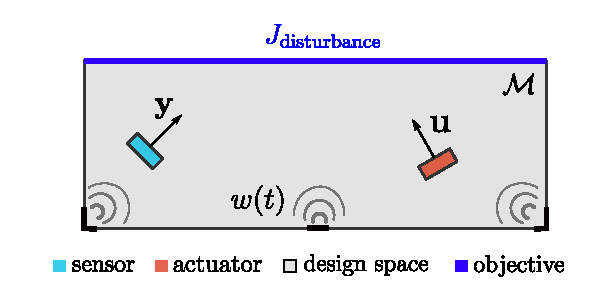
\includegraphics[width=\columnwidth]{./img/drawing2}
  \vspace{-4mm}
  \caption{Example 1: Co-design problem tailored towards finding an optimal morphology $\mathcal{M}$ with internal sensing $\mathbf{y}$ and actuation $\mathbf{u}$ such it suppress the disturbance $w(t)$ at the interface of $\mathcal{M}$. \vspace{-4mm}}
\end{figure}
\begin{figure}[!t]

  \centering
  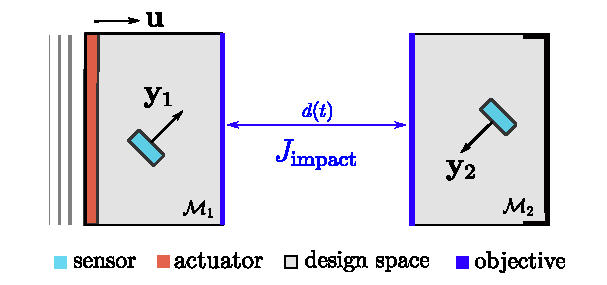
\includegraphics[width=\columnwidth]{./img/drawing3}
  \caption{Example 2: }
  \vspace{-4mm}
\end{figure}

\textbf{Problem formulation.} A (compliant) mechatronic system can be
described by a morphological descriptor
\(\mathcal{M}(\mathcal{G}, \mathsf{B}, \mathsf{M}, \mathsf{K})\), where
\(\mathcal{G}\) denotes the topological graph,
\(\mathsf{B} = \left\{\mathbf{B}_1, ..., \mathbf{B}_n\right\}\)
represents the set of body frames for relevant components (such as
actuators and sensors) with each \(\mathbf{B}_i \in SE(3)\), and
\(\mathsf{M}\), \(\mathsf{K}\), and \(\mathsf{D}\) correspond to the
collections of mass and stiffness of each body frame \(\mathbf{B}_i\).

To facilitate the parametrization of \(\mathcal{M}\), assume the
existence of a decoder function \(E\) that maps a set of continuous
design variables \(\mathbf{\theta}\) to a specific morphological
configuration, i.e., \(E: \mathbf{\theta} \mapsto \mathcal{M}_\theta\).
For each parametrized design \(\mathcal{M}_\theta\), the system's
minimal state representation can be expressed in terms of the state
variables \(\mathbf{x} = (\mathbf{q}, \dot{\mathbf{q}})\) and the
actuation space \(\mathbf{u}\). This formulation yields the structural
dynamics as
\(\dot{\mathbf{x}} = \mathbf{f}(\mathbf{x}, \mathbf{u}; \mathcal{M}_\theta)\)
which may be regarded as an time-evolution encoding given an initial
condition \(\mathbf{x}_0\). An illustrative example of morphological
decoding is given in Fig 3.

As such, we may generalize the co-design problem as a mathematical
optimization of the following form: \begin{equation}
\begin{aligned}
  &\underset{\mathbf{\theta},\,\mathbf{x}(\cdot), \mathbf{u}(\cdot)}{\text{argmin}}
  && \int_{t_1}^{t_2} J(\mathbf{x}(\tau),\mathbf{u}(\tau)) \; d\tau \\
  &\text{subject to}
  && \dot{\mathbf{x}}(t) = f(\mathbf{x}(t), \mathbf{u}(t); \mathcal{M}), \quad \forall t \in [t_1,t_2], \\
  &&& \mathbbf{\theta} \subseteq \mathcal{D}; \;\; \mathbf{x} \subseteq \mathcal{X}; \;\;  \mathbf{u} \subseteq \mathcal{U},
\end{aligned}
\label{eq:optimization_problem}
\end{equation} where \(\mathcal{D}\), \(\mathcal{X}\) and
\(\mathcal{U}\) are the admissible (design) spaces of the morphology,
state trajectories and control action, respectively.

This formulation yields a complex mathematical optimization problem
often characterized by a high-dimensional decision space. Consequently,
careful consideration must be given to decomposing the problem into
computationally tractable subproblems to facilitate efficient solution
strategies.

\textbf{Research scope.} Solving an optimization problem of the form
\ref{eq:optimization_problem} requires a system decomposition of the
problem. The body of research can be categorized in three main topics:

\begin{figure}[!t]
  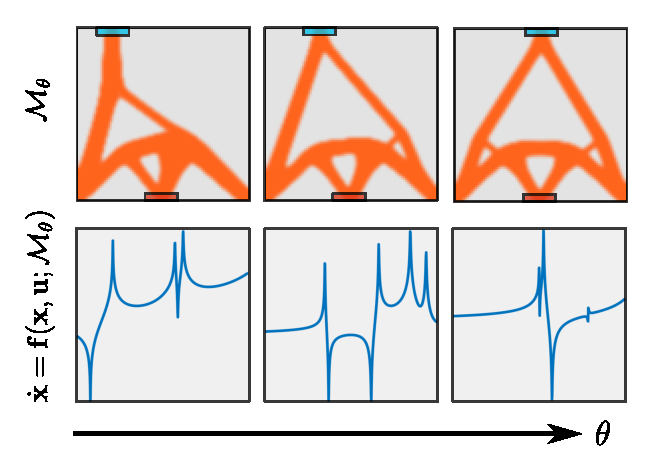
\includegraphics[width=\columnwidth]{./img/drawing}
  \caption{Numerical examples of Karl Sims co-design of artificial-life locomoting creatures}
  \vspace{-4mm}
\end{figure}

\emph{i) Implicit encoding of morphology.} Recent advances in
computational design have introduced implicit encoding techniques for
representing morphology, such as level-set methods, neural implicit
representations and material-point particles. Unlike explicit geometric
models, implicit encodings describe shapes and structures as continuous
functions over spatial domains, enabling flexible and differentiable
parametrization of complex geometries. This approach facilitates smooth
exploration of the design space and supports gradient-based
optimization, which is particularly advantageous for high-dimensional
co-design problems. Moreover, implicit representations allow for direct
integration with simulation and surrogate modeling frameworks, reducing
the need for repeated discretization and accelerating the evaluation of
candidate designs. As a result, implicit encoding has emerged as a
powerful tool for enabling scalable and efficient co-design of compliant
and soft robotic systems.

\emph{ii) Reduced-order dynamics.} Given a morphological description, it
is essential to derive the system's intrinsic dynamics in a
computationally efficient manner. Typically, the underlying physics are
governed by Partial Differential Equations (PDEs), which describe the
evolution of system states over space and time. However, directly
solving high-dimensional PDEs for each design iteration is
computationally prohibitive. To address this, reduced-order modeling
techniques are employed to approximate the system dynamics using a
lower-dimensional set of state variables, preserving essential behavior
while significantly reducing computational cost. Recent advances, such
as neural PDE-refiner methods \cite{lippe2023pderefiner, li2020fourier},
leverage data-driven surrogate models to learn efficient mappings from
design parameters to system responses. These approaches enable rapid
evaluation of candidate morphologies by implicitly encoding the solution
space and bypassing repeated discretization. By selecting appropriate
state variables and constructing reduced-order models, the optimization
process becomes tractable, facilitating scalable co-design of complex
systems with PDE-based dynamics.

Co-design represents a recent paradigm shift in system engineering
frameworks, emphasizing the simultaneous optimization of a mechanical
system's morphology and its associated control strategies to maximize
performance. Unlike traditional design approaches---which often treat
mechanical design and control as sequential, independent
processes---co-design seeks to exploit the synergistic relationship
between structure and control, enabling the development of systems with
superior precision, adaptability, and efficiency.

\input{2_approach.tex}

\bibliographystyle{ACM-Reference-Format}
{\small
\bibliography{references.bib}
}

\end{document}
\endinput
%%
%% End of file `sample-sigconf-xelatex.tex'.


